%----------------------------------------------------------------%
% DOCUMENT CLASS OPTIONS
%----------------------------------------------------------------%
\documentclass[         %
aps,                    %  American Physical Society
prl,                    %  Physical Review D
showpacs,               %  Displays PACS after abstract
%preprint,              %  Preprint layout
%tightenlines,          %  Single spaced lines
superscriptaddress,    %  Authors' addresses linked with superscripts
nofootinbib,            %  Does not treat footnotes as references
%eqsecnum               % 
%onecolumn,             %
twocolumn,             %
showkeys,               %
preprintnumbers,        %
%amsmath,               %
%amssymb,               %
%draft,                 %
%a4paper,               %  A4 paper format
floatfix               %  Fixes float errors
]{revtex4-1}               %  REVTEX 4 Package used
%-----------------------------------------------------------------%
% SOME AVAILABLE PACKAGES
%-----------------------------------------------------------------%
%\usepackage{graphicx,longtable,amsmath}
\usepackage{graphicx,amsmath}
%\usepackage[justification=RaggedRight]{caption}
%\usepackage[justification=justified]{caption}
\usepackage{enumerate}
\usepackage{xcolor}
\usepackage{float}
\usepackage[section]{placeins}
%\usepackage{caption}
\usepackage{subcaption}
\usepackage{amssymb}
\usepackage{commath}
\usepackage{bm}
\usepackage{verbatim}
%-----------------------------------------------------------------%

%\numberwithin{equation}{section}
\renewcommand{\textheight}{9in}
\renewcommand{\topmargin}{0.0in}
%\renewcommand\thesection{\arabic{section}}

% avoids incorrect hyphenation, added Nov/08 by SSR
\hyphenation{ALPGEN}
\hyphenation{EVTGEN}
\hyphenation{PYTHIA}
%-----------------------------------------------------------------%
\begin{document}
%-----------------------------------------------------------------%
\title{Supervised Learning}
%-----------------------------------------------------------------%
%-----------------------------------------------------------------%
\author{Yong-Lin~Zhu}
\email{yzhu459@gatech.edu}
\affiliation{}


%-----------------------------------------------------------------%
\date{\today}
%-----------------------------------------------------------------%
\begin{abstract}
I presents an analysis on the performance of five supervised learning algorithms on two classification problems from UCI datasets,  Mushroom and Adult Income. 
The included algorithms are: Decision Trees, Decision Trees with Adaptive Boosting, k-Nearest Neighbors, Artificial Neural Networks, and Support Vector Machines.
\end{abstract}
%-----------------------------------------------------------------%

\keywords{Machine Learning, Supervised Learning}
%\preprint{}
\maketitle
%------------------------------------------------------------------%

\vskip 1.3cm
%%%%%%%%%%%%%%%%%%%%%%%%%%  Introduction  %%%%%%%%%%%%%%%%%%%%%%%%%%%%%%%%%%%%%%%%%%%%%%
{\bf Introduction}\label{intro}

%Machine Learning is important and popular now.
There are many Supervised Learning algorithms. Discussions(or debates) on which algorithm is better never settles.(see interesting paper in~\cite{fernandez2014we}).

In this manuscript, I will compare five Supervised Learning algorithms on two dataset. The study includes how to split train and test dataset, how to tuning the parameters to get better performance. The best-tuned performance of algorithms on two dataset are discussed at the conclusion. In following sections, I will go through all five algorithms for two dataset in parallel. All the analysis performed here are done with code attached in python and WEKA GUI.

%%%%%%%%% Adult Data
%%%%%%%%% Mushroom Data


{\bf Datasets}\label{datapre}

Both the The Census Income and Mushroom datasets are from the UCI Machine Learning Repository. 

\begin{figure}[h!]
  \centering 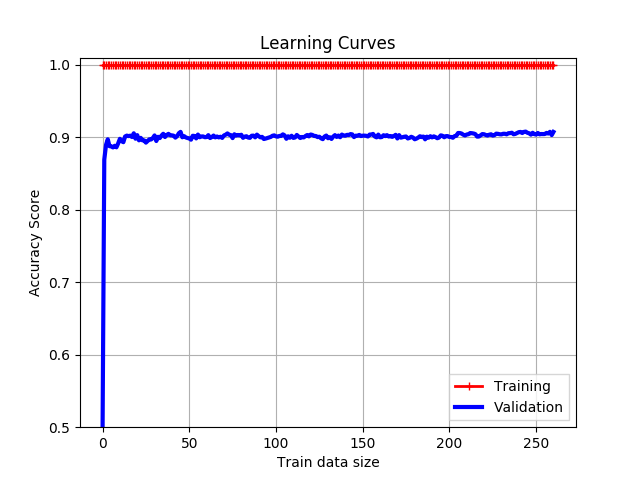
\includegraphics[width=\linewidth]{../DT_adult_LearningCurve}
  \caption{\label{fig:dt_lc_Income}}
\end{figure}

The Census Income dataset(referred as adult in following sections) was extracted by Barry Becker from the 1994 Census database. 
I used this dataset to predict whether a person?s income exceeds $50K$ a year based on their personal information focused on 14 aspects, including age, work class, education, marital status, occupation, race, gender, native county, etc. 
There are eight categorical variables and six continuous variables with 32561 instances. 
The dependent variable, Income has been transformed to a binary variable: 1 means income exceeds $50K/yr$, 0 means not exceeds. 

The Mushroom dataset was drawn from the Audubon Society Field Guide to North American Mushrooms (1981). 
It includes descriptions of hypothetical samples corresponding to 23 species of gilled mushrooms in the Agaricus and Lepiota Family with 23 categorical variables and 8124 instances. 
I used this dataset to predict whether a mushroom is edible or poisonous based on its physical characteristics. 
%%%%%%%%%%%%%%%%%%%%%%%%%%  Decision Tree %%%%%%%%%%%%%%%%%%%%%%%%%%%%%%%%%%%%%%%%%%%%%%
%%%%%%%%%%%%%%%%%%%%%%%%%%    %%%%%%%%%%%%%%%%%%%%%%%%%%%%%%%%%%%%%%%%%%%%%%

{\bf Decision Tree}\label{dt}

%%%%%%%%% Adult Data
In Fig~\ref{fig:dt_lc_Income}, I show the Learning curve for Decision Tree algorithm with the adult data. 
The score of train data is almost constant as training size increases, while the score of the validation set converges to about $0.9$ very fast.
The gap between the lines of training and validation after they converge is because the model has high variance. 
This means the performance of the model may unlikely be constrain by the train size choice. Therefore, I will keep using test dataset as $20\%$ of all. 

\begin{figure}[h!]
  \centering 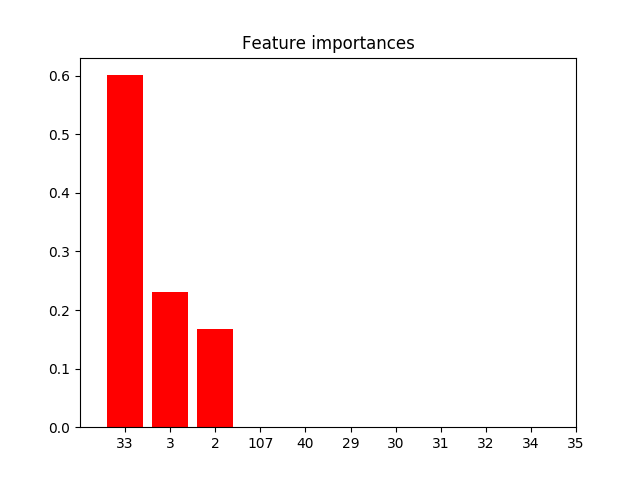
\includegraphics[width=\linewidth]{../FI_income.png}
  \caption{\label{fig:FI_Income}}
\end{figure}

\begin{figure}[h!]
  \centering 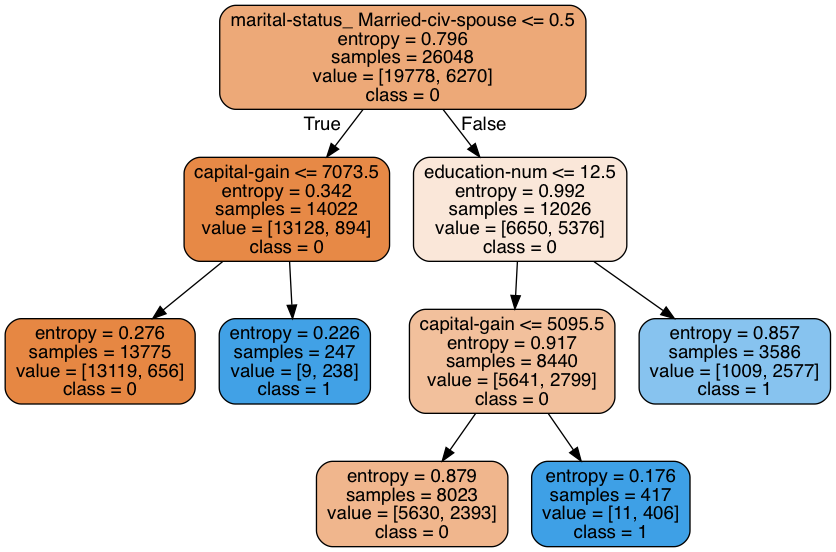
\includegraphics[width=\linewidth]{../dt_income.png}
  \caption{\label{fig:dt_Income}}
\end{figure}

With the default set of max depth of the tree to the number of features, which the the maximum possible, I train this decision tree model first time. Then the top feature importance is shown as in Fig.~\ref{fig:FI_Income}. 
Only $3$ features are much more important than other features, which means one may just need $3$ features to classify most of the dataset.
Therefore, the maximum depth of decision tree will be 4 in our tuned decision tree model. And to keep the tree as small as possible, I set the maximum leaf nodes as $5$ to get the final decision tree as in Fig.~\ref{fig:dt_Income}.


%%%%%%%%% Mushroom Data
\begin{figure}[h!]
  \centering 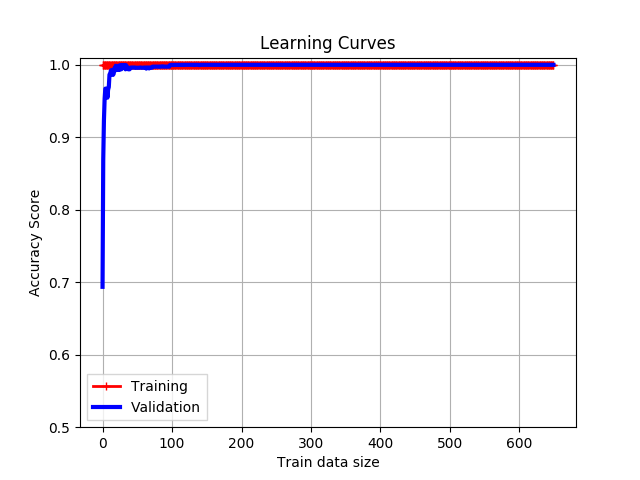
\includegraphics[width=\linewidth]{../DT_mushroom_LearningCurve}
  \caption{\label{fig:dt_lc_mush}}
\end{figure}

\begin{figure}[h!]
  \centering 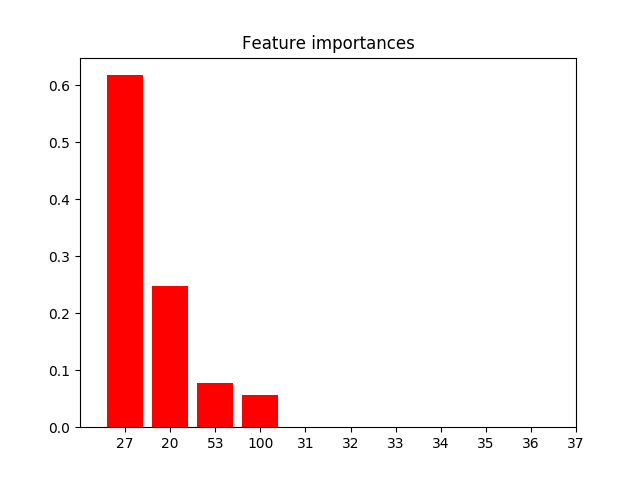
\includegraphics[width=\linewidth]{../FI_mushroom.png}
  \caption{\label{fig:FI_mush}}
\end{figure}

\begin{figure}[h!]
  \centering 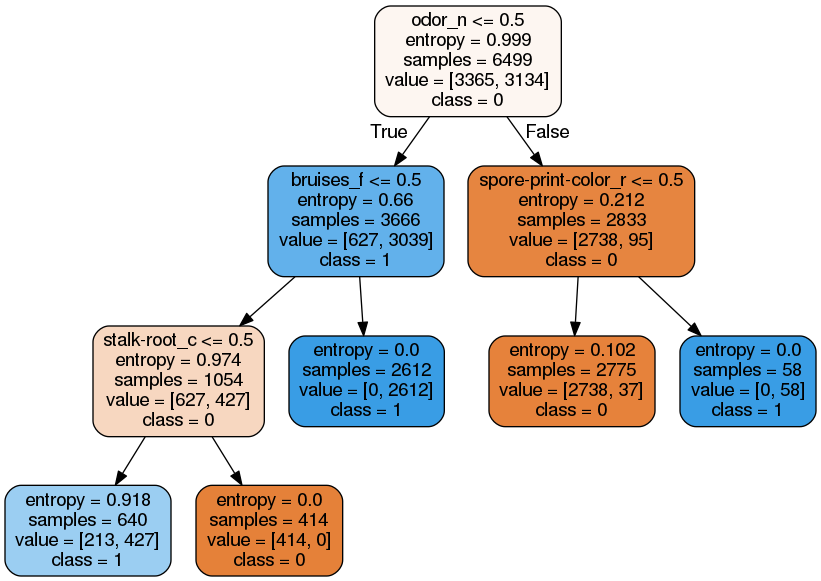
\includegraphics[width=\linewidth]{../dt_mushroom.png}
  \caption{\label{fig:dt_mush}}
\end{figure}

For the mushroom data, In Fig~\ref{fig:dt_lc_mush}, I show the Learning curve for Decision Tree algorithm with the mushroom data. 
The score of train data is almost constant as training size increases, while the score of the validation set converges to about $1$ very fast.
There is no gap between the lines of training and validation after they converge which means that the model has low variance.
This means the performance of the model may unlikely be constrain by the train size choice. Therefore, I will keep using test dataset as $20\%$ of all. 

with similar approach, I set of max depth of the tree to the number of features and train this decision tree model. Then the top feature importance is shown as in Fig.~\ref{fig:FI_mushroom}. 
Only $4$ features are much more important than other features, which means one may just need $4$ features to classify most of the dataset.
Therefore, the maximum depth of decision tree will be 5 in our tuned decision tree model. 
And to keep the tree as small as possible, I set the maximum leaf nodes as $5$ with maximum depth as $4$ to get the final decision tree as in Fig.~\ref{fig:dt_mushroom}.

%%%%%%%%%%%%%%%%%%%%%%%%%%  NN %%%%%%%%%%%%%%%%%%%%%%%%%%%%%%%%%%%%%%%%%%%%%%
%%%%%%%%%%%%%%%%%%%%%%%%%%    %%%%%%%%%%%%%%%%%%%%%%%%%%%%%%%%%%%%%%%%%%%%%%
{\bf Neural networks}\label{nn}

Neural networks can be very complicated in most cases. 
One can vary the learn rates, hidden layer, nodes in each layer, etc.
It is not like other algorithms with which one can try the parameters with brute force within limited times of attempts. 
So here, instead of searching the best parameters, I will just suggest one handed tuned neural network and validate its performance.
I start with three layers and vary the number of node from 2 to 10 nodes in each layer. 
After a handful of runs, I use three hidden layers with 4 nodes in each layer as the final neural network. 
In Fig.\ref{fig:ANN_lc_adult}, I plot the accuracy score of training and validation set as a validation curve.
%%%%%%%%% Adult Data%%%%%%%%%%%%%%%%%%%%%%%%%%%%%%%%%%%%%%%%%%%%%%

\begin{figure}[h!]
  \centering 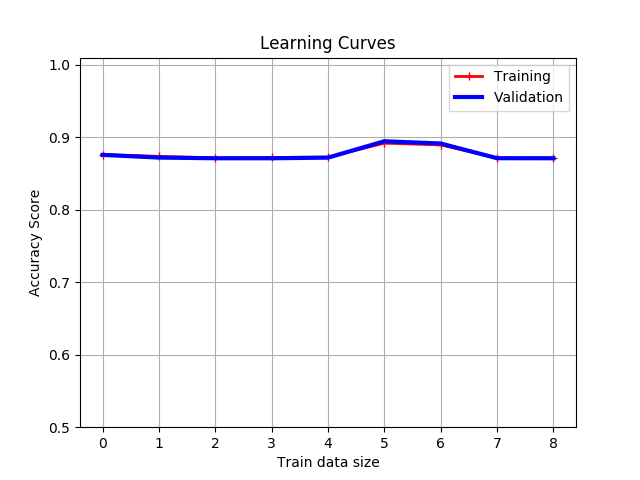
\includegraphics[width=\linewidth]{../ANN_adult_LearningCurve.png}
  \caption{ANN Adult LearningCurve.\label{fig:ANN_lc_adult}}
\end{figure}

The decision tree model on mushroom data performs very well as the accuracy score reaches almost $100\%$. 
It seem there is a definite relationship in the features and outcome.
The neural network is good at dealing with more complex problems.
In Fig.~\ref{fig:ANN_lc_mush}, not surprisingly the accuracy score converges to $100\%$ very fast. 
Here I used the same layer and nodes as for the adult. 
I am sure there is much simpler network.
But there is not much to improve for modeling on this dataset.
%%%%%%%%% Mushroom Data
\begin{figure}[h!]
  \centering 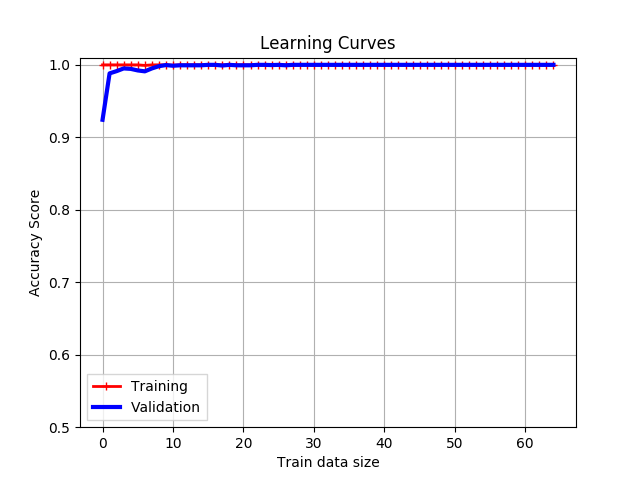
\includegraphics[width=\linewidth]{../ANN_mush_LearningCurve.png}
  \caption{ANN Mushroom LearningCurve.\label{fig:ANN_lc_mush}}
\end{figure}

%%%%%%%%%%%%%%%%%%%%%%%%%%  Boosting %%%%%%%%%%%%%%%%%%%%%%%%%%%%%%%%%%%%%%%%%%%%%%
%%%%%%%%%%%%%%%%%%%%%%%%%%    %%%%%%%%%%%%%%%%%%%%%%%%%%%%%%%%%%%%%%%%%%%%%%

{\bf Boosting}\label{boost}

Here I boost the Decision Tree trained above. For the adult data, I have get the tuned and pruned parameters, as setting the maximum leaf nodes to $5$ and maximum depth to $4$.
Compared to the unboosted model in Fig.~\ref{fig:dt_lc_Income}, the boosted model has smaller gap in the line of accuracy scores for training and validating set.
This means the boosted model has lower variance than the unboosted model. The boosting clearly improves the model performance.
%%%%%%%%% Adult Data
\begin{figure}[h!]
  \centering 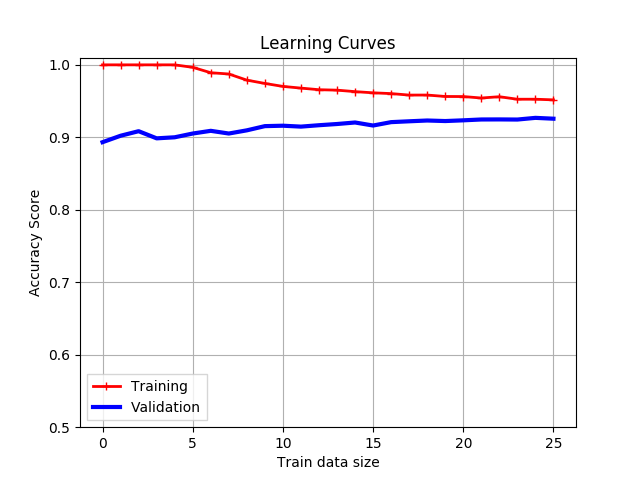
\includegraphics[width=\linewidth]{../boosting_adult_LearningCurve}
  \caption{Boosting Adult Learning Curve\label{fig:svmrbf_lc_adult}}
\end{figure}

Similarly, I used the Decision Tree model trained above for the mushroom dataset.
The unboosted Decision Tree works very well in Fig.~\ref{fig:dt_lc_mush}. 
The boosted Decision Tree converges even faster in Fig.~\ref{fig:svmrbf_lc_mush}
%%%%%%%%% Mushroom Data\\
\begin{figure}[h!]
  \centering 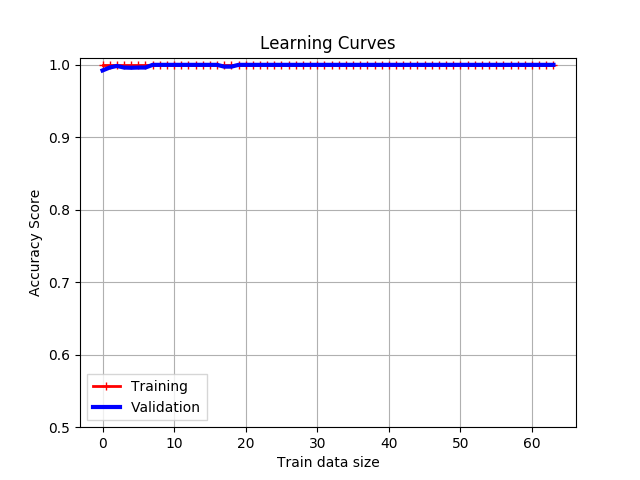
\includegraphics[width=\linewidth]{../boosting_mush_LearningCurve}
  \caption{Boosting Mushroom Learning Curve\label{fig:svmrbf_lc_mush}}
\end{figure}

%%%%%%%%%%%%%%%%%%%%%%%%%%  SVM %%%%%%%%%%%%%%%%%%%%%%%%%%%%%%%%%%%%%%%%%%%%%%
%%%%%%%%%%%%%%%%%%%%%%%%%%    %%%%%%%%%%%%%%%%%%%%%%%%%%%%%%%%%%%%%%%%%%%%%%
{\bf Support Vector Machines}\label{svm}
I use two different kernels here linear kernel and rbf for Support Vector Machines.
In Fig.~\ref{fig:svmrbf_lc_adult,fig:svml_lc_adult}, the gap between two lines are bigger than any one from other algorithms.
The models of SVM are not very good for this dataset since they come with high variance.
%%%%%%%%% Adult Data
\begin{figure}[h!]
  \centering 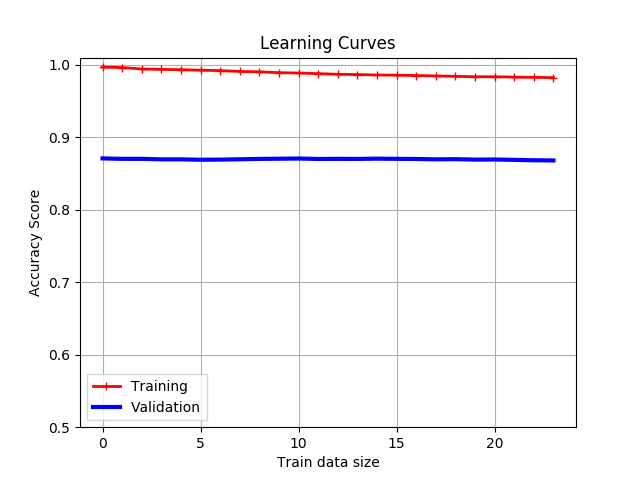
\includegraphics[width=\linewidth]{../svm_income_LearningCurve_rbf}
  \caption{SVM Adult RBF Learning Curve\label{fig:svmrbf_lc_adult}}
\end{figure}

\begin{figure}[h!]
  \centering \includegraphics[width=\linewidth]{../svm_income_LearningCurve_linear}
  \caption{SVM Adult Linear Learning Curve\label{fig:svml_lc_adult}}
\end{figure}
%%%%%%%%% Mushroom Data
Although this data set is very fast to train and all the models so far perform very well, I find that the linear kernel here converges faster than the RBF kernel.
\begin{figure}[h!]
  \centering 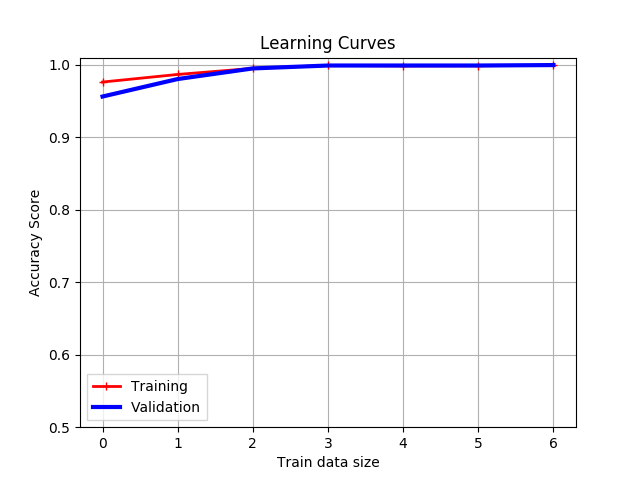
\includegraphics[width=\linewidth]{../svm_mushroom_LearningCurve_rbf}
  \caption{SVM Mushroom RBF Learning Curve\label{fig:svmrbf_lc_mush}}
\end{figure}

\begin{figure}[h!]
  \centering 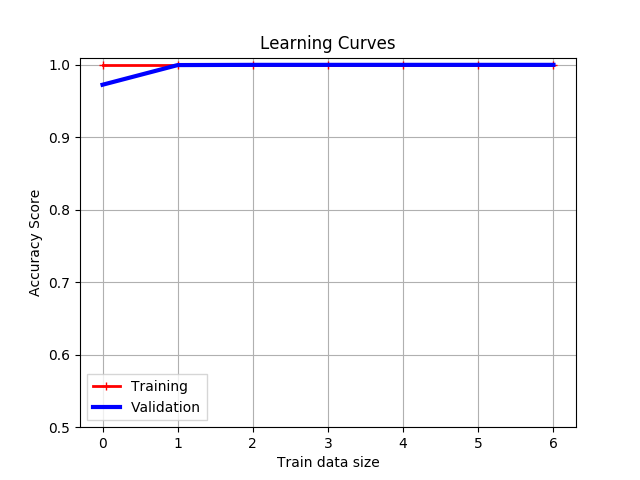
\includegraphics[width=\linewidth]{../svm_mushroom_LearningCurve_linear}
  \caption{SVM Mushroom Linear Learning Curve\label{fig:svml_lc_mush}}
\end{figure}

%%%%%%%%%%%%%%%%%%%%%%%%%%  KNN %%%%%%%%%%%%%%%%%%%%%%%%%%%%%%%%%%%%%%%%%%%%%%
%%%%%%%%%%%%%%%%%%%%%%%%%%    %%%%%%%%%%%%%%%%%%%%%%%%%%%%%%%%%%%%%%%%%%%%%%
{\bf k-nearest neighbors}\label{knn}

%%%%%%%%% Adult Data
For the mushroom data, In Fig~\ref{fig:knn_lc_adult}, I show the Learning curve for k-nearest neighbors algorithm with the adult data. 
The score of train data and the validation set converge quickly together but to different value around 0.9. 
This means the performance of the model may unlikely be constrain by the train size choice. Therefore, I will keep using test dataset as $20\%$ of all. 
There is obvious gap between the lines of training and validation after they converge which means that the model has high variance.
\begin{figure}[h!]
  \centering 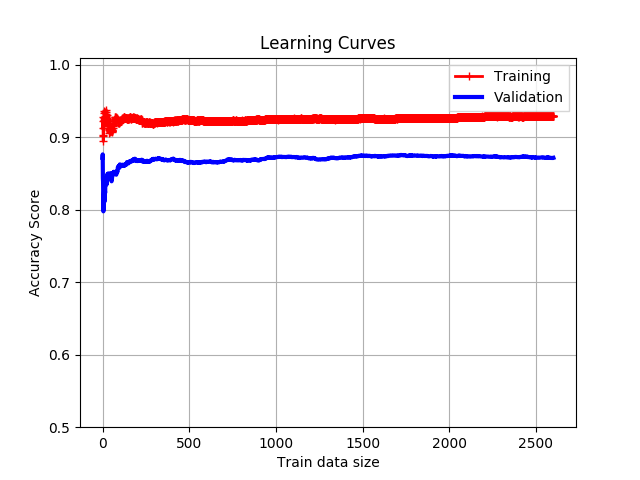
\includegraphics[width=\linewidth]{../knn_adult_LearningCurve}
  \caption{KNN Adult LearningCurve\label{fig:knn_lc_adult}}
\end{figure}
For the k-nearest neighbors, the k is a key parameter.
Typically k is odd when the number of classes is 2, which is the case in this adult classification problem. 
To find the best k for the model, I compute the misclassification error vs k in Fig.\ref{fig:knn_adult}
\begin{figure}[h!]
  \centering \includegraphics[width=\linewidth]{../knn_adult}
  \caption{KNN\label{fig:knn_adult}}
\end{figure}
%%%%%%%%% Mushroom Data
For the mushroom data, In Fig~\ref{fig:knn_lc_mush}, I show the Learning curve for k-nearest neighbors algorithm with the mushroom data. 
The score of train data and the validation set converge quickly together to about $1$ very fast. 
This means the performance of the model may unlikely be constrain by the train size choice. Therefore, I will keep using test dataset as $20\%$ of all. 
There is no gap between the lines of training and validation after they converge which means that the model has low variance.
\begin{figure}[h!]
  \centering 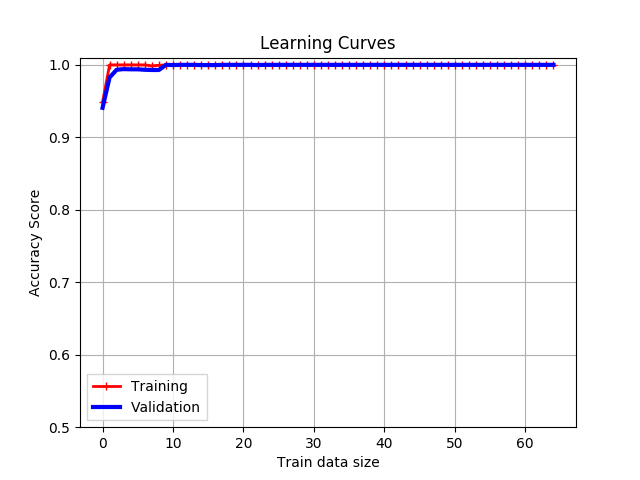
\includegraphics[width=\linewidth]{../knn_mush_LearningCurve}
  \caption{KNN Mushroom LearningCurve \label{fig:knn_lc_mush}}
\end{figure}
For the k-nearest neighbors, the k is a key parameter.
Typically k is odd when the number of classes is 2, which is the case in this mushroom classification problem. 
To find the best k for the model, I compute the misclassification error vs k in Fig.\ref{fig:knn_mush}
\begin{figure}[h!]
  \centering \includegraphics[width=\linewidth]{../knn_mushroom}
  \caption{\label{fig:knn_mush}}
\end{figure}

% Commands to include a figure:
{\bf Conclusion \label{conclusion}}
For the classification problem on the adult data, the performance of different algorithms varies. 
The SVM in Fig.~\ref{fig:svmrbf_lc_adult,fig:svml_lc_adult} show the largest gap between training and validation set. 
And the accuracy scores is below $88\%$.
The boosted Decision Tree gives the best accuracy score over $92\%$ and the gap between training and validation is the smallest.
But in general, all the five algorithms give accuracy score around $90\%$. 
In conclusion, the boosted Decision Tree model is the best in terms of accuracy score and variance.

The mushroom classification is a very interesting one for me. I personally love wild mushroom as food.
But I don't have much knowledge about which mushroom is eatable or not. 
In this problem, I try to used the five algorithm to find a model that can classify the mushroom into eatable or not. 
All five models perform very good and even some of them achieve $100\%$ accuracy score. 
Normally I will guess that there may be overfitting with such high accuracy score. 
However, I train the models with cross-validation and check on the learning curves.
In conclusion, all the five model give a great classification on the mushroom problem.
%\input acknowledgement.tex   % input acknowledgement
\bibliographystyle{apsrev4-1}
\bibliography{ref.bib}

\end{document}